%@+leo-ver=4-thin
%@+node:paran.20140515173914.6982:@shadow Background.tex
%@@color
%@@language latex
\chapter{Background}

As this thesis is about maintaining private views within a version control system what follows is some background concerning version control systems and how they determine if a change has occurred in source code.  
We will also cover refactoring before looking more closely at JDime and other tools that attempt to reduce merge conflicts caused by refactoring or reformatting.  

\section{Version Control Systems}
%@<<VersionControlSystems>>
%@+node:paran.20140528183434.1974:<<VersionControlSystems>>
%@<<Reasons for using version control>>
%@+node:paran.20140530135904.1945:<<Reasons for using version control>>
Version control systems are a way of managing different revisions (or versions). 
Version control systems can be used to keep revisions of files that are in any format. 
Most commonly they are used for maintaining source code written for a plain text programming language (e.g. Java, C, etc.). 
There are a number of reasons why we might want to use a version control system. It can be used to refer to previous revisions, to maintain a revision that has an experimental feature, to associate additional documentation about a feature or to collaborate with multiple developers who are on the same programming project:

\begin{description}

  \item [Revisit revisions using tagging.]
  %@  <<revisions>>
  %@+node:paran.20140530135904.1948:<<revisions>>
  A version control system can be used by a single person to manage different revisions of their program. 
  A previous revision can always be revisited at a later date and changed. 
  If there is something significant about a particular revision it can be labelled with a \emph{tag}. 
  A tag assigns a name to all the files in the revision you are interested in so that you can more easily revisit the code at a certain point.  
  This is helpful if a software package has a number of released versions.  
  If you need to go back and revisit a particular release it becomes a lot easier if you have tagged the code at that point with the release name or other identification.
   
   

  %@-node:paran.20140530135904.1948:<<revisions>>
  %@nl
  
  \item [Use branching for experimental features.] 
  %@  <<branching>>
  %@+node:paran.20140530135904.1950:<<branching>>
  It is also possible to maintain multiple revisions of all the files for a software project. 
  This is useful if there is an experimental feature which you want to explore but want to maintain the original as a separate project. 
  As shown in Figure ~\ref{fig:bgBranches} a version control system can keep these multiple interests separate by putting them on different \emph{branches}. 
  It is still possible to easily switch between the different branches depending on which project you want to make changes to.  
  A good use of this feature is if you have a software project that you have written on behalf two different companies but each of them would like their own unique customisations on top of the base product.  
  By making two copies of the base product and having a record of when it was divided the branches can later be recombined to include some or all of the features that have been introduced.  

  \begin{figure}[!t]
   \begin{center}
    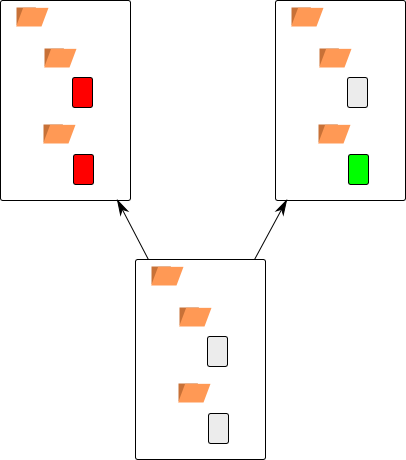
\includegraphics[scale=.8]{branching}
   \end{center}
   \caption{A project that has been split into two branches. Both the red files have been changed for the left branch whilst only the green one has changed in the right branch.}
   \label{fig:bgBranches}
  \end{figure}

  %According to Willaims \cite{Williams2008} branching and merging still is complex and it is hard to get good results from a text-based merge.
  %@-node:paran.20140530135904.1950:<<branching>>
  %@nl

  \item [Attach documentation to a feature.]
  %@  <<associating metadata>>
  %@+node:paran.20140530135904.1951:<<associating metadata>>
  Another useful feature of version control is the ability to record meta information beside changes to a set of files.
  The reason this is useful is that you can specify what the change was for.
  It is possible to associate a change that has occurred over multiple files as being for the same reason.
  Most version control systems allow a message to be written when documents are checked in.
  In some version control systems this message is required.
  The reason this is useful is for when queries are made about what a certain change to a document was for.
  Since there is a message beside all the documents about the reason for a particular change it becomes easier to figure out the reason for the individual change we are interested in. 
  %@+at
  % If following the example above we were to examine a document and wonder 
  % why the address changed we could examine the check in with that change and 
  % see the message that the person changing it wrote.
  %@-at
  %@@c

  \begin{figure}[!t]
   \begin{center}
    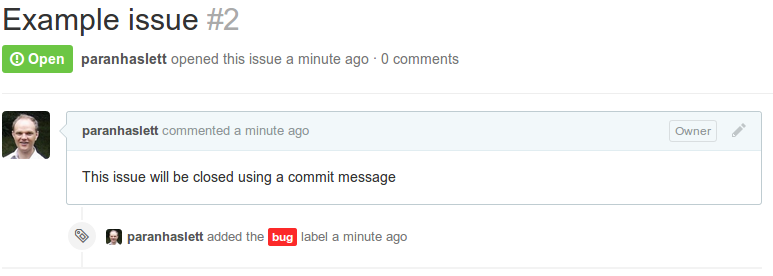
\includegraphics[scale=.5]{bugtrack}
   \end{center}
   \caption{A issue that has been created in GitHub}
   \label{fig:bgBugTrack}
  \end{figure}

  When used on source code in tandem with an \emph{bug tracking system} the message can contain the identification number for the bug being fixed or feature being added.
  This means that anybody who is examining the revision to see the reasoning for the change has access to a lot more information via the bug tracking system.
  An example of this is the \emph{issue tracker} that is built in to GitHub, an online version control system. In GitHub an issue (e.g. a bug report or feature request) can be created as shown in Figure ~\ref{fig:bgBugTrack}. 
  The issue tracker is linked with the messages that you need to write when you check in files.
  If you include a hash sign followed by an issues' identification number in the message you check in then GitHub updates that issue, as shown in Figure ~\ref{fig:bgBugUpdate}.

  \begin{figure}[!t]
   \begin{center}
    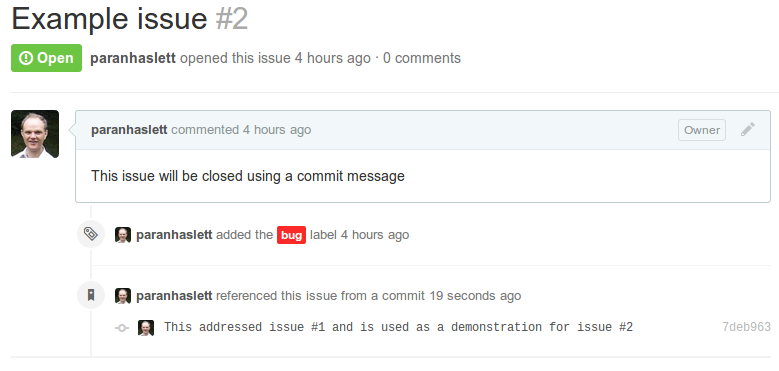
\includegraphics[scale=.5]{bugupdate}
   \end{center}
   \caption{The issue has been updated using a commit message}
   \label{fig:bgBugUpdate}
  \end{figure}
  %@nonl
  %@-node:paran.20140530135904.1951:<<associating metadata>>
  %@nl

  \item [Collaborate with multiple developers.]
  %@  <<collaboration>>
  %@+node:paran.20140530135904.1949:<<collaboration>>
  Version control systems make it possible to have individual revisions that contain each person's changes. 
  The version control system then manages the way these changes are merged into a composite product. 
  Bertino \cite{Bertino2012} describes the ability to merge the work of multiple people as being a powerful collaborative tool. 
  This is because a version control system allows multiple people with different ideas to collaborate on the same document. 
  In some circumstances it allows them to work on the document at the same time. This feature seems similar to the concept of having a private view that we are exploring in this thesis. The difference is that a version control system has no awareness about the format of the documents. This means it is harder for it to evaluate the difference between features of the document that will be helpful to collaboration and features that express the individual tastes of each of the collaborators.
  %@-node:paran.20140530135904.1949:<<collaboration>>
  %@nl

\end{description}


%@-node:paran.20140530135904.1945:<<Reasons for using version control>>
%@nl

\subsection{Dealing with conflicts}
%@<<LockvsMerge>>
%@+node:paran.20140529075353.1935:<<LockvsMerge>>
When people work on the same software project there is a need to interact with each other.
If they require the same source code then there is competition to access that file for each of them to successfully do their work.
There is the risk that they will attempt to change the same block of source code at the same time.
If different changes are made to the same block of source code then they have a \emph{merge conflict} and need to figure out how to combine the changes manually.
There are a few ways of dealing with these conflicts.

\subsubsection{Locking}
%@<<locking>>
%@+node:paran.20140530135904.1952:<<locking>>
One approach is to require that a file is only able to be used by one person at a time and that anyone else has to wait. This method avoids the need to resolve any conflicting changes.  The advantage of locking a file like this is that it is that we can be certain about the contents of the file at any given time. This is how one of the original version control systems, RCS ensured that the document stayed consistent. Tichy \cite{Tichy1982} has explained why he considers locking in a version control system to be a good idea in the design for RCS. The disadvantage is if one person retains the document for extended periods of time, it cannot be changed by anybody else. Furthermore the resulting document may be barely recognisable as the original if extensive work is done on it. However, if the two parties change distinctly different parts of the file, or both independently make exactly the same changes this restriction is unnecessary. 
%@nonl
%@-node:paran.20140530135904.1952:<<locking>>
%@nl
\subsubsection{Smaller structured units}
%@<<reduction>>
%@+node:paran.20140529174111.1936:<<reduction>>
Another way to reduce conflicts is to split the programming code into smaller units.  The advantage of this is that if you are using locking you minimise the risk that two people need access to the same unit of source code. Consider two people working on the same project made up of a number of files.  Instead of one person locking a file at a time that person could be allowed to only lock the functions they are changing. As those functions are smaller than the file there is likely to be less changes and they are likely to unlock them sooner.
%@nonl
%@-node:paran.20140529174111.1936:<<reduction>>
%@nl
\subsubsection{Merging documents}
%@<<Merging>>
%@+node:paran.20140528183434.2055:<<Merging>>
Finally we could allow both parties to change the document and try to figure out what the problems are afterwards.  This resolution of anything that remains a problem is known as resolving a \emph{merge conflict}. This occurs whenever the computer cannot automatically process a merge.  The merge then needs to be sorted out manually. Merge conflicts are more likely to occur if there is a dramatic change such as refactoring.

If not regularly merged it is possible for the source code to diverge greatly and it becomes harder and harder to reconcile.
 According to Bertino it is possible to keep a smaller more easily deployed repository by excluding files that can be generated. \cite{Bertino2012}. Although Bertino refers to unnecessary files this premise may also be applicable for the smaller blocks of code we are interested in. This suggests that maintaining a record about what is relevant and what is irrelevant may have some benefit (e.g. the non-functional changes).
 
\begin{description}
  \item [Manual Merging.]
%@<<Manual Merging>>
%@+node:paran.20140528183434.2056:<<Manual Merging>>
If you have two files you want to merge but no common starting point for them both you will need to manually merge any differences.
The computer has no record about what the original file looked like so it can not determine which changes were intended.
Features that they have in common will not need to be affected however a decision needs to be made about any differences by the developers responsible for those changes.

%@+at
% insert diagram
%@-at
%@@c
%@nonl
%@-node:paran.20140528183434.2056:<<Manual Merging>>
%@nl
  \item [Automatic Merging.] 
%@<<Automatic Merging>>
%@+node:paran.20140528183434.2057:<<Automatic Merging>>
An automatic merge is possible if three revisions are available, the original revision, the revision containing changes we have made and the revision containing changes made by other developers. 
By comparing the differences between our revision and the original one it is possible to determine which changes we have made.  
If we compare the changes made by other developers to the original, the changes that they have made can be determined.  
If we attempt to update our code by merging other people's changes and a change only occurs in our code then that change is retained. 
If we attempt to update our code by merging other people's changes and a change only occurs in the other persons code the the change is inserted into our code.
A merge conflict can however still occur when a change is made in the same area of code in both revisions.
The merge conflicts need to be dealt with manually.


%@+at
% Diagram showing that how merging could be done automatically
% if there is a change in your code but no change in others code automatic
% if there is a change in others code but not yours
% 
%@-at
%@@c
%@nonl
%@-node:paran.20140528183434.2057:<<Automatic Merging>>
%@nl
\end{description}
 


%@+at
%   Version control still can have problems with merge conflicts.
%@-at
%@@c 
%@nonl
%@-node:paran.20140528183434.2055:<<Merging>>
%@nl
%@nonl
%@-node:paran.20140529075353.1935:<<LockvsMerge>>
%@nl

\subsection{Types of version controls systems}
%@<<architecture>>
%@+node:paran.20140530135904.1946:<<architecture>>
\begin{description}

  \item [Centralised version control.] 
  %@  <<Centralised Version control>>
  %@+node:paran.20140528183434.2058:<<Centralised Version control>>
  In a centralised version control system all the changes are made to one location.
  This is called a centralised repository.
  Having a centralised repository means that only one place needs to be checked in order to access the most up-to-date and agreed upon source code.
  The need to be connected to a central system allowed multiple developers the ability to work on the same source code but often had a large overhead.
  Some centralised systems required a specialist to be involved just to look after the server and ensure that merges were done correctly.
  However according to Chacon \cite{Chacon2009} this single point of management has some advantages as it is possible to manage what developers had access to. 
  According to Chacon \cite{Chacon2009} and Bertino \cite{Bertino2012} the main flaw with centralised version control systems is that they have a single point of failure.
  If anything goes wrong with the server you could lose all your work.

  %@-node:paran.20140528183434.2058:<<Centralised Version control>>
  %@nl
  \item [Distributed version control.] 
  %@  <<Distributed Version control>>
  %@+node:paran.20140528183434.2059:<<Distributed Version control>>
  According to Chacon \cite{Chacon2009} and Bertino \cite{Bertino2012} this is like having a complete copy of a repository present on every computer that has access to that project

  One advantage of having a complete copy of a project from the repository are that it eliminates the single point of failure that centralised version control systems have.
  It also makes it possible to make changes to the program remotely without being connected to a central server.
  At a later time you are able to merge you changes with other people's work.  
  You are also able to select changes others have made and incorporate them into your personal copy.

  %@+at
  % NOTE: put more in here if time
  %@-at
  %@@c
  %@-node:paran.20140528183434.2059:<<Distributed Version control>>
  %@nl
  \item [Online version control systems.]  
  %@  <<GitHub>>
  %@+node:paran.20140603140023.2025:<<GitHub>>
  Whilst is is possible for a measure of collaboration just by using a version control system on its own, it requires that you have some method of obtaining the separate branches on one machine before they can be merged.
  One way of doing this within a company is to set up a server for the version control system.
  This might be suitable for projects that are closed source and have a select group of people who work on the source code.
  For larger projects that have programmers in different parts of the world a publicly accessible version control system that is on the web may be a better solution.
  Loeliger \cite{Loeliger2006} shows how it is possible to access and use a web based version control system to achieve this.
  A good example of a web based version control system is GitHub.
  GitHub provides a way for many developers in different parts of the world to change source code for an open source project.
  It is possible that the developers for a particular project have not even met in real life or even know about each other.

  As an example we could look at the JGit.
  JGit is a pure Java implementation of the Git version control system.
  Figure ~\ref{fig:bgUsage} shows part of the GitHub page for JGit highlighting the amount of activity that there has been on the JGit project.
  With 74 contributors supplying 3245 changes means that the potential to have conflicting changes must be high. Having 20 separate branches may indicate that merges often need to happen. This one example could indicate the need for good merge tools that can reconcile conflicts even if the developers have little contact with each other.

  \begin{figure}[!t]
   \begin{center}
    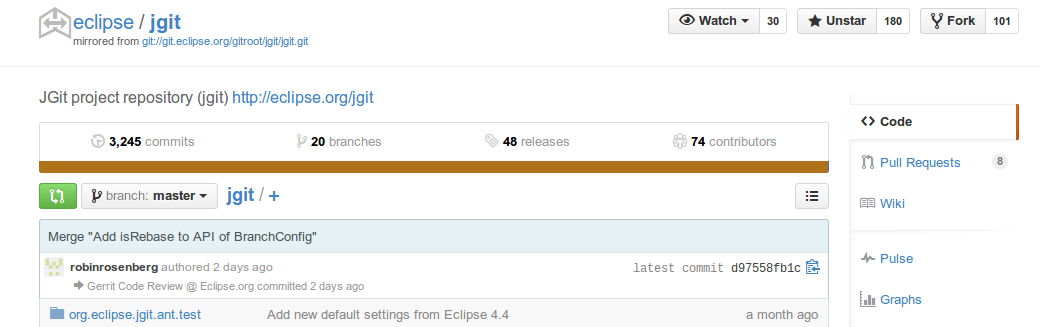
\includegraphics[scale=.47]{githubUsage}
   \end{center}
   \caption{The overview page of the Jgit project in GitHub. This shows that there are 74 contributors to the source code and 3245 individual changes over 20 branches.}
   \label{fig:bgUsage}
  \end{figure}


  %@-node:paran.20140603140023.2025:<<GitHub>>
  %@nl
  
\end{description}
%@nonl
%@-node:paran.20140530135904.1946:<<architecture>>
%@nl
%@-node:paran.20140528183434.1974:<<VersionControlSystems>>
%@nl

\section{Longest Common Subsequence}
%@<<LCS>>
%@+node:paran.20140528183434.2009:<<LCS>>
The longest common subsequence problem is relevant to this thesis as it concerns comparing code to determine similarities and differences.
The similarities and differences can then be used to automatically merge code in a version control system.

A simple definition of the longest common subsequence problem is attempting to find the maximum number of common items in two strings when the strings are examined from left to right. A subsequence does not need to be in a single contiguous block however. Algorithms that solve the longest common subsequence can determine the differences between two lists by working out what is the same.   


\subsection{Example}
%@<<Example of Longest common subsequence>>
%@+node:paran.20140528183434.2010:<<Example of Longest common subsequence>>
\label{sec:examplelcs}

An example of finding the longest common subsequence is as follows.
Imagine we have two similar sets of Java source code that we want to compare with each other.  
We would like to know what is the same and what is different.
A longest common subsequence for the source would contain a list of all the lines that are the same and in the same order.


\begin{minipage}[t]{1.0\textwidth}
The first listing is as follows:

%\begin{figure}[!t]
\begin{lstlisting}
%@<<first listing>>
%@+node:paran.20140812094111.2155:<<first listing>>
public class SampleLCS {
  public static double area(double radius){
    return Math.PI * square(radius);
  }
  
  public static void main(String[] args){
    System.out.println(area(3));
  }
 
  public static double square(double num){
    return num * num;
  }
}
%@nonl
%@-node:paran.20140812094111.2155:<<first listing>>
%@nl
\end{lstlisting}
\end{minipage}
%\end{figure}

\begin{minipage}[t]{1.0\textwidth}
In the second listing the order of a number of methods has changed but the way the code works has not been changed.

%\begin{figure}[!t]
\begin{lstlisting}
%@<<second listing>>
%@+node:paran.20140812094111.2156:<<second listing>>
public class SampleLCS {
  public static void main(String[] args){
    System.out.println(area(3));
  }
 
  public static double square(double num){
    return num * num;
  }
 
  public static double area(double radius){
    return Math.PI * square(radius);
  }
}
%@nonl
%@-node:paran.20140812094111.2156:<<second listing>>
%@nl
\end{lstlisting}
\end{minipage}
%\end{figure}

\begin{minipage}[t]{1.0\textwidth}
A listing containing only the common lines in the same order between both listings follows.  Since this is one of the longest listings possible it is known as the longest common subsequence.  

%\begin{figure}[!t]
\begin{lstlisting}
%@<<first lcs>>
%@+node:paran.20140812094111.2157:<<first lcs>>
public class SampleLCS { 
  public static double area(double radius){
    return Math.PI * square(radius);
  }
  
}
%@nonl
%@-node:paran.20140812094111.2157:<<first lcs>>
%@nl
\end{lstlisting}
\end{minipage}
%\end{figure}

\begin{minipage}[t]{1.0\textwidth}
It is possible to have more than one longest common subsequence if there are multiple listings of common lines that have the same number of lines in common and have the maximum number of lines that match.  For instance the following listing is also a longest common subsequence of the above example.

%\begin{figure}[!t]
\begin{lstlisting}
%@<<second LCS>>
%@+node:paran.20140812094111.2158:<<second LCS>>
public class SampleLCS {
  public static void main(String[] args){
    System.out.println(area(3));
  }
 
}
%@nonl
%@-node:paran.20140812094111.2158:<<second LCS>>
%@nl
\end{lstlisting}
\end{minipage}
%\begin{figure}

As there are possibly multiple longest common subsequences identifying the longest common subsequence that is going to be most useful becomes difficult.
%@nonl
%@-node:paran.20140528183434.2010:<<Example of Longest common subsequence>>
%@nl

\subsection{Methods of calculating LCS}
%@<<Git difference strategies>>
%@+node:paran.20140528183434.2011:<<Git difference strategies>>
According to Arslan \cite{Arslan2010} there are many algorithms that solve longest common subsequence problem. As is it possible for there to be multiple correct solutions to a LCS problem a reason for having a different algorithm may be to find the LCS that make the most intuitive sense. The algorithms used in JGit (an open source implementation of Git in Java) for example are the the Myers, Patience and Histogram algorithms. JGit predominately uses the Histogram algorithm with a fall-back of using the Myers algorithm as a fall-back if it gets to computationally expensive.  There is also the option of using the Patience algorithm however this will produce similar results to the Histogram algorithm which has been derived from it. 

%@<<Myers>>
%@+node:paran.20140528183434.2012:<<Myers>>
\subsection{Myers}
The Myers algorithm was discovered by Eugene Myers \cite{Myers1986} who claimed that finding the minimal differences between any two documents was the equivalent to finding the shortest or longest path in a graph.

%For example if we have two ...

% explain how this is achieved 
%@-node:paran.20140528183434.2012:<<Myers>>
%@nl

%@<<Patience>>
%@+node:paran.20140528183434.2013:<<Patience>>
\subsection{Patience}
The patience algorithm instead of figuring out the longest common subsequence directly uses the longest increasing subsequence. 
The example used by Aldous \cite{Aldous1999} to explain how the Patience algorithm finds the longest increasing subsequence is similar to a single player card game.
The aim of the game is to create the minimal number of piles of cards in a row.
A higher card may not be placed on a pile with a lower one in it.
Cards need to be placed on the leftmost valid pile. 
A new pile needs to be created at the end of the row for any cards that cannot be placed on any existing pile.
This game discovers the longest increasing subsequence of the cards when they were shuffled before the game is played.
The cards in the pile to the immediate left of each card when it is played are all possible elements that could come before it in a longest increasing subsequence.
By taking notes of the card on top of of the pile to the immediate left whenever a card is played a longest subsequence can be calculated.     

The Patience algorithm only detects \emph{markers} which are matching lines of code that appear only once in both revisions of the source code.
By using the Patience algorithm on line numbers for the markers instead of on cards the longest common subsequence can be established for those markers. 

As Bram Cohan \cite{bramcohen} has pointed out in his blog there are instances where a traditional LCS algorithm can return results that although correct are not as helpful as they could be.
This is especially true when there are multiple possible longest common subsequences.
The patience algorithm initially ignores lines that appear multiple times and focuses first on solving the longest common subsequence problem for the markers, which only appear once. 
By doing this it has a clearer picture about where to place the lines that occur multiple times.
%@-node:paran.20140528183434.2013:<<Patience>>
%@nl

%@<<Histogram>>
%@+node:paran.20140528183434.2014:<<Histogram>>
\subsection{Histogram}
The patience algorithm works well when there are matches that only occur once in both revisions, but has difficulty in determining what to do if line only appear more than once.
It is possible to fall back on a Myers algorithm for the segments where multiple matches occur, however it is possible for Myers to produce unhelpful results. 
The Histogram algorithm attempts to overcome this by also detecting lines that occur in both revisions a small number of times.
The algorithm is solely used in JGit at the moment and is a derivative of the Bram Cohens patience algorithm. 
More details about this algorithm can be found in the Javadoc for HistogramDiff in the JGit source code \cite{Foundation2014}. 


% Before determining a LCS the 
%@nonl
%@-node:paran.20140528183434.2014:<<Histogram>>
%@nl
%@-node:paran.20140528183434.2011:<<Git difference strategies>>
%@nl

\subsection{How LCS is used in differencing tools}
%@<<How diffs use LCS>>
%@+node:paran.20140528183434.2016:<<How diffs use LCS>>
Differencing tools (often shortened to "diff tools") are programs that compare the contents of two files and show the similarities and differences.
In many diff tools a hash code is assigned to each line of the files to speed up the differencing process.
This means that the differencing tool can work much faster as it does not need to compare each character in the line but can compare hash codes instead.
However the granularity of what is compared is more coarse as it shows complete line differences rather than word or character differences. 
In the source code for many programming languages the white space is not relevant so many diff tools have the option of ignoring the white space and only comparing the code.
This has an impact on the hash codes for each line as the hash code needs to be generated just from the text without including white spaces.

Additionally with some diff tools it is possible to use regular expressions to ignore program features such as comments when doing a diff.  The reason this is important is if it is possible exclude changes that have no affect on behaviour from a diff then it is possible to also exclude them from a merge.  If we exclude them from a merge we could have fewer conflicts.

%@+at
% insert examples of this with references semantic merge maybe
%@-at
%@@c
%@nonl
%@-node:paran.20140528183434.2016:<<How diffs use LCS>>
%@nl

\subsection{The problem with LCS}
%@<<The problem with LCS>>
%@+node:paran.20140528183434.2015:<<The problem with LCS>>
From the perspective of this thesis there is still a problem with longest common subsequence. 
It does not notice changes of order in a document.  
For the example in section \ref{sec:examplelcs} two methods that have swapped positions.
The program still behaves in the same manner when it is run.
It is unnecessary to make any changes to this code in order to get them to behave the same way.
Diff tools that solely use the longest common subsequence do not take different ordered items into account even if they can be considered equivalent.

\begin{figure}[h]
\begin{center}
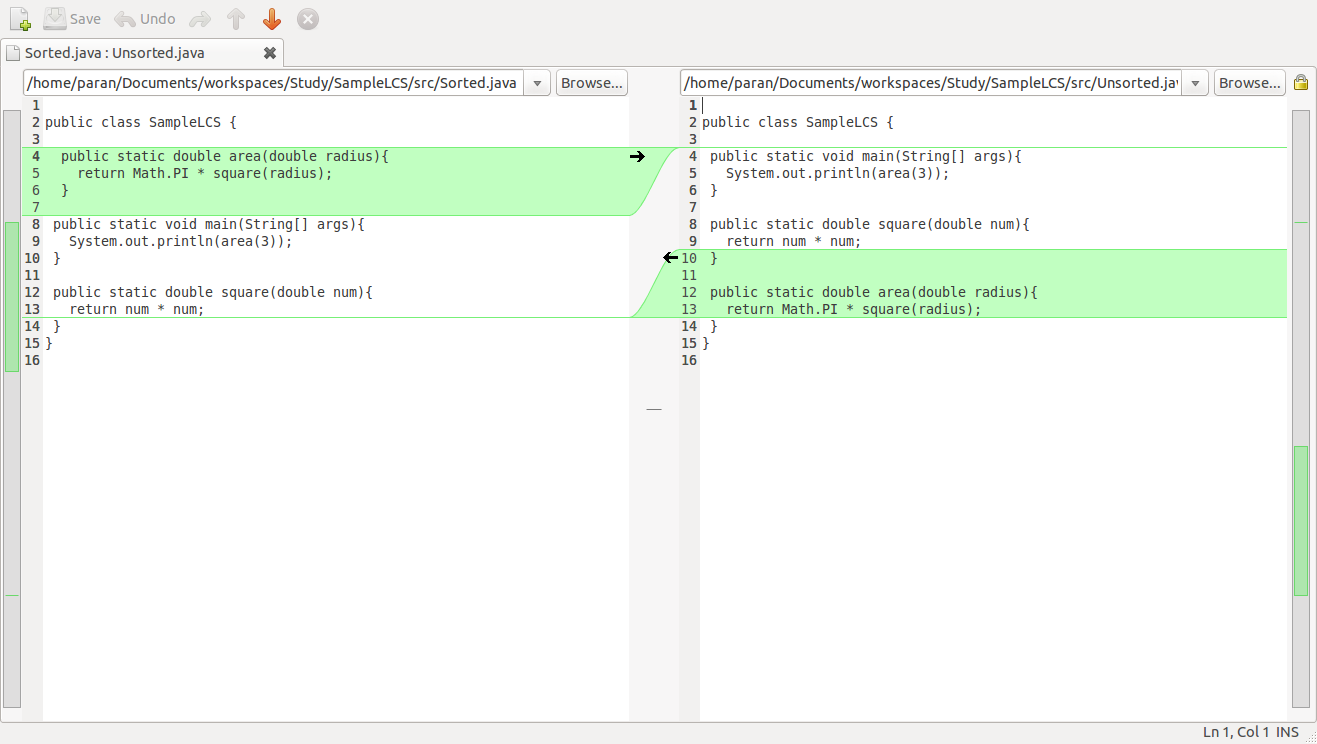
\includegraphics[scale=.28]{lcsDiff}
\end{center}
 \caption{A graphical diff tool showing differences with two equivalent blocks of source code}
\end{figure}
%@-node:paran.20140528183434.2015:<<The problem with LCS>>
%@nl


 
%@-node:paran.20140528183434.2009:<<LCS>>
%@nl

\section{Refactoring}
%@<<Refactoring>>
%@+node:paran.20140530135904.1958:<<Refactoring>>
A common concern with coding is the need to periodically refactor the code. 
When we use the word refactored here we refer to the definition of refactoring presented by Murphy-Hill \cite{Murphy-Hill2008} who claims that refactoring simply changes the structure of the code but not the behaviour.
Refactoring simply reorganises the source code so that it is easier to read and add changes. 
According to Fowler et al. the main time for refactoring is when new functionality is added \cite{Fowler1999}. 
Similarly according to Kerievsky some of the motivations for refactoring include adding more code and understanding existing code \cite{Kerievsky2004}.
As adding more functionality is one of the motivations for refactoring let us consider what happens in a multi-developer environment. 
Two developers could have different views on what is considered an appropriate refactoring. 
This is especially true if they need to add different functionality from each other. 
We will now demonstrate this with the following two code examples:

\begin{minipage}[t]{1.0\textwidth}
%\begin{figure}[!t]
\begin{lstlisting}
public TempConv() {
  %@  <<tempConv>>
  %@+node:paran.20140530135904.1959:<<tempConv>>
  Scanner keyboard = new Scanner(System.in);
  System.out.println("Enter the temperature in Celsius");
  int celsius = keyboard.nextInt();
  System.out.println("Degrees Fahrenheit is approx " 
    + (celsius * 2 + 30) );
  keyboard.close();
  %@nonl
  %@-node:paran.20140530135904.1959:<<tempConv>>
  %@nl
}
\end{lstlisting}
%\end{figure}
\end{minipage}


Refactoring this code depends on what functionality you need to add. 
One developer may recognize that conversion from Celsius may be used several times throughout the code and so extract the calculations as a separate method as follows:

\begin{minipage}[t]{1.0\textwidth}
%\begin{figure}[!t]
\begin{lstlisting}
public TempConv() {
  %@  <<tempConv2>>
  %@+node:paran.20140530135904.1960:<<tempConv2>>
  Scanner keyboard = new Scanner(System.in);
  System.out.println("Enter the temperature in Celsius");
  int celsius = keyboard.nextInt();
  System.out.println("Degrees Fahrenheit is approx " 
    + celsiusToFahrenheit(celsius));
  keyboard.close();
  %@nonl
  %@-node:paran.20140530135904.1960:<<tempConv2>>
  %@nl
}

public int celsiusToFahrenheit(int celsius){
  %@  <<celsiusToFahrenheit>>
  %@+node:paran.20140530135904.1961:<<celsiusToFahrenheit>>
  return celsius * 2 + 30;
  %@nonl
  %@-node:paran.20140530135904.1961:<<celsiusToFahrenheit>>
  %@nl
}
\end{lstlisting}
%\end{figure}
\end{minipage}

This change, in spite of producing the same output as the first, provides a number of advantages. Firstly if other programs need to convert from Celsius to Fahrenheit the new method can easily be reused. Secondly since the calculation is a crude estimation it becomes a lot clearer where the code needs to be changed to improve the formula. The ability to add a method that clearly indicates that the calculation is from Celsius to Fahrenheit helps with the readability of the code. There are also disadvantages to doing this refactoring. If we do not care about conversion between Celsius and Fahrenheit the refactoring simply adds to the amount of code we need to examine before understanding what the code does. An alternative way of refactoring is as follows:

\begin{minipage}[t]{1.0\textwidth}
%\begin{figure}[!t]
\begin{lstlisting}
public TempConv(){
  %@  <<tempConv3>>
  %@+node:paran.20140530135904.1962:<<tempConv3>>
  Scanner keyboard = new Scanner(System.in);
  System.out.println("Enter the temperature in Celsius");
  int celsius = keyboard.nextInt();
  int celsiusToFahrenheit = celsius *2 + 30;
  System.out.println("Degrees Fahrenheit is approx " 
    + celsiusToFahrenheit);
  keyboard.close();
  %@nonl
  %@-node:paran.20140530135904.1962:<<tempConv3>>
  %@nl
}
\end{lstlisting}
%\end{figure}
\end{minipage}

While this again expresses the same functionality as the code above it has not created a new method to do so. This has some of the same advantages. It separates and identifies the formula to convert between Celsius and Fahrenheit. It also uses less code to express this separation than forming a new method. It does not expose the conversion formula outside this method to be used by other calculations however.

As the value of a particular refactoring appears to depend on what is trying to be achieved it is very hard to claim that one refactoring is better than another. Rather, it depends on the wider context of the intention for the refactoring, in this case the level of access required for the approximation to convert Celsius to Fahrenheit.

Although this was a simple example it is easy to imagine a case where a much larger refactoring process is undertaken. In such circumstances a merge becomes difficult. 
%@-node:paran.20140530135904.1958:<<Refactoring>>
%@nl

\section{JDime}
%@<<JDime>>
%@+node:paran.20140528183434.2021:<<JDime>>
%@+at
% Part of the inspiration for this tool come from JDime.
%@-at
%@@c

JDime is a tool written by  Apel and Le{\ss}enich \cite{Apel2012} \cite{Apel2011} \cite{LeBenich2012} to study how to get a balance between fast text-based merges and slow but more accurate semantic merges.  JDime is designed to merge two sets of code even if both of them have undergone refactoring. It does this by parsing the class files into AST and evalutating the AST for a \emph{semantic merge} In order to increase performance only if there is a conflict in a text based merge does any of the more expensive semantic merge take place. 

\subsection{How JDime works}
%@<<How Jdime works>>
%@+node:paran.20140528183434.2023:<<How Jdime works>>
%@+at
% JDime instead of testing against a source code repository test against files 
% in the system under the base, left and right directories.
% While this may be useful in quickly being able to show what JDime is able to 
% achieve it requires that the inputs need to be previously extracted from a 
% repository into the file system.
%@-at
%@@c

Before doing any calculations, JDime runs a regular text merge over the source code.  
If the regular text merge has conflicts then JDime parses the file into an abstract syntax tree (AST).  JDime uses the AST to determine if sections of the source code need to be in a particular order or could be in any order.
What then happens depends on if order is required in the section of code JDime is examining.

%@+at
% needs more here
%@-at
%@@c
%@nonl
%@-node:paran.20140528183434.2023:<<How Jdime works>>
%@nl

\subsection{Investigating JDime}
%@<<Testing Jdimes suitability>>
%@+node:paran.20140528183434.2024:<<Testing Jdimes suitability>>
We performed a small experiment to investigate JDime as a tool for automatically merging code which has been reordered.
%@+at
% As JDime can examine many refactorings and do comparisons between two 
% private views of source code it is a good contender for allowing us to 
% create two separate views that have different refactorings in them.  However 
% we want the views to remain as consistent as possible. This means we do not 
% want the structure of one view to change the structure of another view if 
% they have the same behaviour when the code is executed.  Any changes to 
% functionality should be able to be communicated between views however 
% changes that are ascetic should not affect the other view.  For this reason 
% we want to test JDimes suitability to be one of the tools used to create 
% separate refactored views.
% 
% JDime has been written mostly in Java.  There are a few exceptions including 
% the linear programming libraries that need to be created.  As we are 
% attempting to combine some of their work with Git it was decided to use JGit 
% rather than the C implementation of Git. As the Java implementation may run 
% a bit slower then in order to get a good timing test running we need to run 
% redo the tests of JDime using JGit instead.
% 
% Also the tests that Le{\ss}enich did on JDime were from files rather than 
% from a repository. It is necessary to set the files back up in the original 
% repository structure to get a adequate baseline.
%@-at
%@@c
As JDime performs a type of automatic merge it requires 3 different revisions.
JDime requires a revision that has changes that we want included.  This is commonly called the right revision however I will call this the merger revision as the changes in it are meant to be merged.
JDime also requires a revision that we want to merge into.  This is commonly called the left revision, however I will refer to this as being the mergee. 
Finally JDime requires an original revision that both the merger and the mergee are based on.
This is commonly called the base revision.
%@+at
% At the moment it cannot access a version control system so each of the 
% revisions need to be set up as directories.
% Each directory needs a full copy of the source code for that revision
% This means that the necessary Java source code to be used by JDime in base, 
% left and right directories.
%@-at
%@@c

In order to show how JDime performs extra refactoring based merging we need to attempt to try something that would incorrectly cause a conflict in a text based merge.  The reason that this is necessary is that if there are no conflicts in a text based merge the refactoring aware portion of JDime will not be run.  This saves the overhead of loading the program into an AST in the event that the initial text merge has no conflicts. 
One way to get a lot of text conflicts between two pieces of code that are equivalent when they run is to change the order of the methods.
Although the methods are in different order the programs are still "functionally equivalent".
In order to examine how JDime works and test its suitability a test handler was written.
The test handler creates all of the directories and files for JDime to process.
The methods inside the files are reordered differently for both the left and the right directories.
Figure ~\ref{fig:bgJDimeTest} demonstrates how the test files were arranged.


\begin{figure}[!t]
\begin{center}
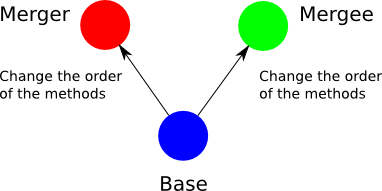
\includegraphics[scale=1]{JdimeTestSetup}
\end{center}
 \label{fig:bgJDimeTest}
 \caption{The set-up for the test of JDime}
\end{figure}

Once the test was set up using the test handler the JDime run to process the directories.
What we expected to happen was that JDime would reorder the methods to match the order in the mergee. As shown in Figure ~\ref{fig:bgJDimeScreenShot} When we compared the methods using a graphical merge tool however we found that the order of the methods in the files did not match.

\begin{figure}[!t]
\begin{center}
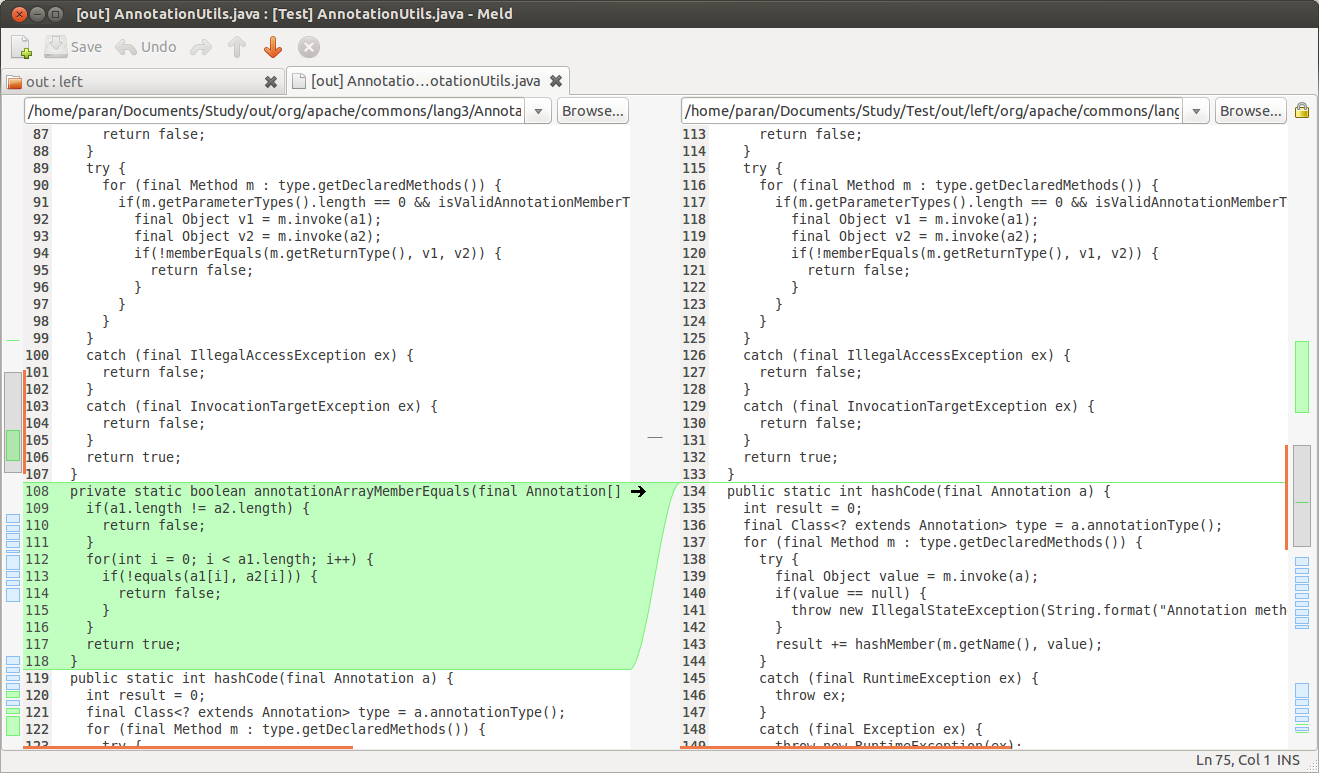
\includegraphics[scale=0.25]{DiffLeft}
\end{center}
 \label{fig:bgJDimeScreenShot}
 \caption{Screen-shot of Meld showing a different method order}
\end{figure}


Further investigation revealed that the order of the methods in the final merged code example did not match the order of any of the equivalent input files.    
In other words JDime normalises its output so that methods are in a particular order.
%@+at
% If it detects an unordered section it does not preserve the order of the 
% output.
%@-at
%@@c
%@nonl
%@-node:paran.20140528183434.2024:<<Testing Jdimes suitability>>
%@nl

\subsection{Reasons why JDime cannot currently be used to create separate views}
%@<<Conclusion>>
%@+node:paran.20140604093616.2026:<<Conclusion>>
The aim of this thesis is to be able to maintain two views of Java that, although having a different format, function in the same manner.  Although JDime seems like it would be able to help achieve those aims there are a few reasons why it cannot be used without changes.

%@<<first issue>>
%@+node:paran.20140605091816.2391:<<first issue>>
The first issue is that as explained above that the merged code could be in a totally different order to the original file and both of the revisions.
%@nonl
%@-node:paran.20140605091816.2391:<<first issue>>
%@nl

%@<<second issue>>
%@+node:paran.20140605091816.2392:<<second issue>>
The second issue is that when JDime parses the code into an AST it strips out any comments or white-space placed in the code.  Although the comments do not have any functional impact on how the program runs they do have an impact on how the source code is understood.  To limit the impact a merge makes on one view comments need to be evaluated as well. In some ways retaining comments or even white-space in the code aids in determining if a section of the code has been copied verbatim from one place to another.
%@nonl
%@-node:paran.20140605091816.2392:<<second issue>>
%@nl

%@<<third issue>>
%@+node:paran.20140605091816.2394:<<third issue>>

%@+at
% The only time an AST based merge is performed in JDime is if there are plain 
% text conflicts.  However there could be a hidden conflict that the plain 
% text merge does not detect.  For example if we have two different views and 
% a method has both been relocated in both of them.  Although the method in 
% the original version is in the middle of the code one revision relocates it 
% near to the top of the file and the other to the bottom.  If in addition to 
% this a change is introduced inside the method in both revisions that would 
% normally produce a conflict had the method not been moved.
% 
% A text based merge would not recognise this as a conflict however a AST 
% based one would. According to the text based merge both revisions would 
% agree that the method had been deleted from the middle of the file.  One 
% revision however would insist that a new method with the same name as the 
% deleted one has been created near the top of the file.  The other revision 
% would insist that a new method with the same name had been created but near 
% the bottom. When merged both the method at the top and method at the bottom 
% would be inserted into the merged code.
% 
% A merge using an AST would recognise the methods described as being a 
% conflicting change.  As the names and method signature has not changed for 
% either method it would recognise the conflicting change that has been 
% introduced.
% 
% As JDime does not use an AST comparison to check any items that have been 
% deemed non-conflicting by the text based merge it would miss this conflict.
%@-at
%@@c

%@+at  
% According to the text-merge  There could be advantage to determining if 
% items that haven't conflicted in the text based merge but have moved from 
% one position in the code to another.  If a method has both been moved and 
% changed in both branches it could have a conflict.  This conflict would 
% appear to the text-merge as a deletion agreed upon by both branches followed 
% by two insertions at different points.  It would not be picked up by the 
% text-merge as containing a conflict even if one was potentially present.  
% Since the conflict is not detected by a text-merge it is not set aside for 
% testing by examining the AST tree. In this case comparing AST trees could 
% detect that there was a conflict. Although JDime is an improvement over a 
% text-based merge this is a potential conflict that neither detect. There is 
% a performance reason for this design decision. JDime can take a long time to 
% determine if two files contain equivalent source code.
%@-at
%@@c
%@nonl
%@-node:paran.20140605091816.2394:<<third issue>>
%@nl

%@<<final issue>>
%@+node:paran.20140605091816.2393:<<final issue>>
The final concern is that after JDime does the initial comparison of text and finds conflicts it discards those results. It parses the entire file into an AST and begins analysing it again without knowing which parts differ.   
%@nonl
%@-node:paran.20140605091816.2393:<<final issue>>
%@nl
%@-node:paran.20140604093616.2026:<<Conclusion>>
%@nl

%@-node:paran.20140528183434.2021:<<JDime>>
%@nl
\section{Other refactoring aware versioning tools}
%@<<oravt>>
%@+node:paran.20140731220748.2056:<<oravt>>
JDime is not the only tool that can be used to address refactor aware version control.  Ekman and Asklund \cite{Ekman2004} introduced a plug-in for eclipse that recorded information about refactoring in to version control so that it was easier to recognise where refactoring took place.  They did this in a very similar manner as Apel and Le{\ss}enich when they developed JDime.  Both make use of an AST to record information about any refactoring that took place.  Freese \cite{Freese2006} also developed a tool that was very similar written in Object-Z. Despite this interest in refactoring aware merges however the idea of maintaining private views has not been discussed.
%@nonl
%@-node:paran.20140731220748.2056:<<oravt>>
%@nl
%@-node:paran.20140515173914.6982:@shadow Background.tex
%@-leo
